\documentclass[12pt, a4paper, twocolumn]{article}

\usepackage{graphicx} % Required for inserting images
\usepackage[T1]{fontenc}
\usepackage[utf8]{inputenc}
\usepackage{microtype} % améliorations microtypographiques
\usepackage[english]{babel}
\usepackage{csquotes}
\usepackage{xcolor}
\usepackage{epigraph}
\usepackage{subcaption}
\usepackage{authblk}
\usepackage{url} 
\usepackage{soul}
\usepackage{hyperref}
\usepackage{makecell}
\usepackage{booktabs}  % nice looking tables
\usepackage{numprint}
\usepackage[title]{appendix}

\usepackage[newfloat]{minted}
\newenvironment{code}{\captionsetup{type=listing}}{}
\SetupFloatingEnvironment{listing}{name=Code}

\usepackage{sectsty}  % font size
\sectionfont{\fontsize{15}{15}\selectfont}

\usepackage{amsmath} 
\usepackage{mathtools} 
\newcommand\scalemath[2]{\scalebox{#1}{\mbox{\ensuremath{\displaystyle #2}}}}

\renewcommand{\arraystretch}{1.3}%vertical spacing between table rows

\usepackage{acro}
\DeclareAcronym{iiif}{%
    short=IIIF,%
    long=International Image Interoperability Framework%
}
\DeclareAcronym{fair}{%
    short=FAIR,%
    long={Findable, Accessible, Interoperable, Reusable}%
}
\DeclareAcronym{gis}{%
    short=GIS,
    long={Geographical Information System}%
}

%\usepackage[acronym]{glossaries}
%\setacronymstyle{short-long}
%\newacronym{fair}{FAIR}{Findable, Accessible, Interoperable, Reusable}
%\newacronym{iiif}{IIIF}{International Image Interoperability Framework}


\usepackage[backend=biber, style=authoryear,sorting=ynt]{biblatex}
\addbibresource{includes/jdmdh_richelieu.bib}

\definecolor{amethyst}{rgb}{0.6, 0.4, 0.8}
\definecolor{outrageousorange}{rgb}{1.0, 0.43, 0.29}
\definecolor{fashionfuchsia}{rgb}{0.96, 0.0, 0.63}
\definecolor{guppiegreen}{rgb}{0.0, 1.0, 0.5}

\providecommand{\keywords}[1]{
  \noindent\small	
  \textbf{\textit{Keywords---}} #1
}
\providecommand{\basiccomment}[2]{
    %\colorbox{#1}{\texttt{#2}}
    \begingroup
    \sethlcolor{#1}%
    \hl{#2}
    \endgroup

}
\providecommand{\commentcharlotte}[1]{
    \basiccomment{fashionfuchsia}{CHARLOTTE: #1}
}
\providecommand{\commentcolin}[1]{
    \basiccomment{guppiegreen}{COLIN: #1}
}
\providecommand{\commentpaul}[1]{
    \basiccomment{outrageousorange}{PAUL: #1}
}

\title{Accessing urbanity through art historical sources: a situated digital humanities approach}
\author[1]{\textbf{Charlotte Duvette}}
\author[2]{\textbf{Paul Kervegan}}
\author[3]{\textbf{Colin Prudhomme}}
\affil[1]{
    École nationale supérieure d'architecture de Bretagne}
\affil[2]{
    LIGM, École des Ponts, IP Paris, UGE, CNRS}
\affil[3]{
    École nationale des chartes et École Centrale de Lille}

%\date{February 2025}

\begin{document}

\maketitle

\begin{abstract}
We propose that images are a central historical source to gain a better understanding of urbanity in the \textit{quartier Richelieu} (Paris, France) during a period of unprecedented media production (1750-1950). Urban phenomena are mutli-faceted -- everyday practices as well as urban planning structure space in a relationship with an economical, architectural and political framework. These phenomena are then approached through a wide array of digital tools: a GIS and 3D modeling are used to map evolutions in the plot plan, before confronting iconography to the architectural space; a multi-modal data model aims to position our sources within a network of relationships that structure the neighbourhood. While our approach aims at exhaustivity, it is highly localized: focusing on a handful of streets allows us to develop a situated perspective on digital tools, while attempting to identify the dynamics at play in the production of a neighbourhood in a 19\textsuperscript{th} century European capital.
\end{abstract}

\keywords{Architecture, art history, visual culture, iconography, interdisciplinarity, database modeling, interface design, IIIF, API, 3D modeling
}

\section{Introduction to the creation of a digital image ecosystem: between digital humanities and art history}
\subsection{\textit{Richelieu. Histoire du quartier}}

Since November 2024, the Web platform of the research project \textit{Richelieu: Histoire du quartier (1750-1950)}\footnote{Richelieu: History of a neighbourhood}  is  accessible online\footnote{\url{https://quartier-richelieu.inha.fr}}. It contains 4217 digitized iconographic documents from 26 institutions, representing 1118 named entities and 331 places spatialized in a digital map. In addition to the sources and their metadata, there are 14 short research articles. Through a data enrichment process, the project's researchers transformed an iconographic database into complex network: tens of thousands of relations between the neighbourhood's images and other entities were identified,  offering new ways  of understanding the multidimensional nature of the historic city. 

This Web platform is the culmination of a pivotal phase in our research project, initiated in 2019 from a collaboration among several public institutions based in the heart of Paris . The aim was to examine a cluster of Parisian streets known as the \textit{Richelieu} neighbourhood (fig. \ref{fig:outline}), delving into their architectural, human, and economic dynamics through a comprehensive analysis of historic, iconographic and cartographic sources. Our goal was to uncover what makes this neighborhood both ``unique'' and ``representative'' in the 19\textsuperscript{th}-century city, us
ing insights from art history, architecture, and digital humanities.

\begin{figure}[h]
    \centering
    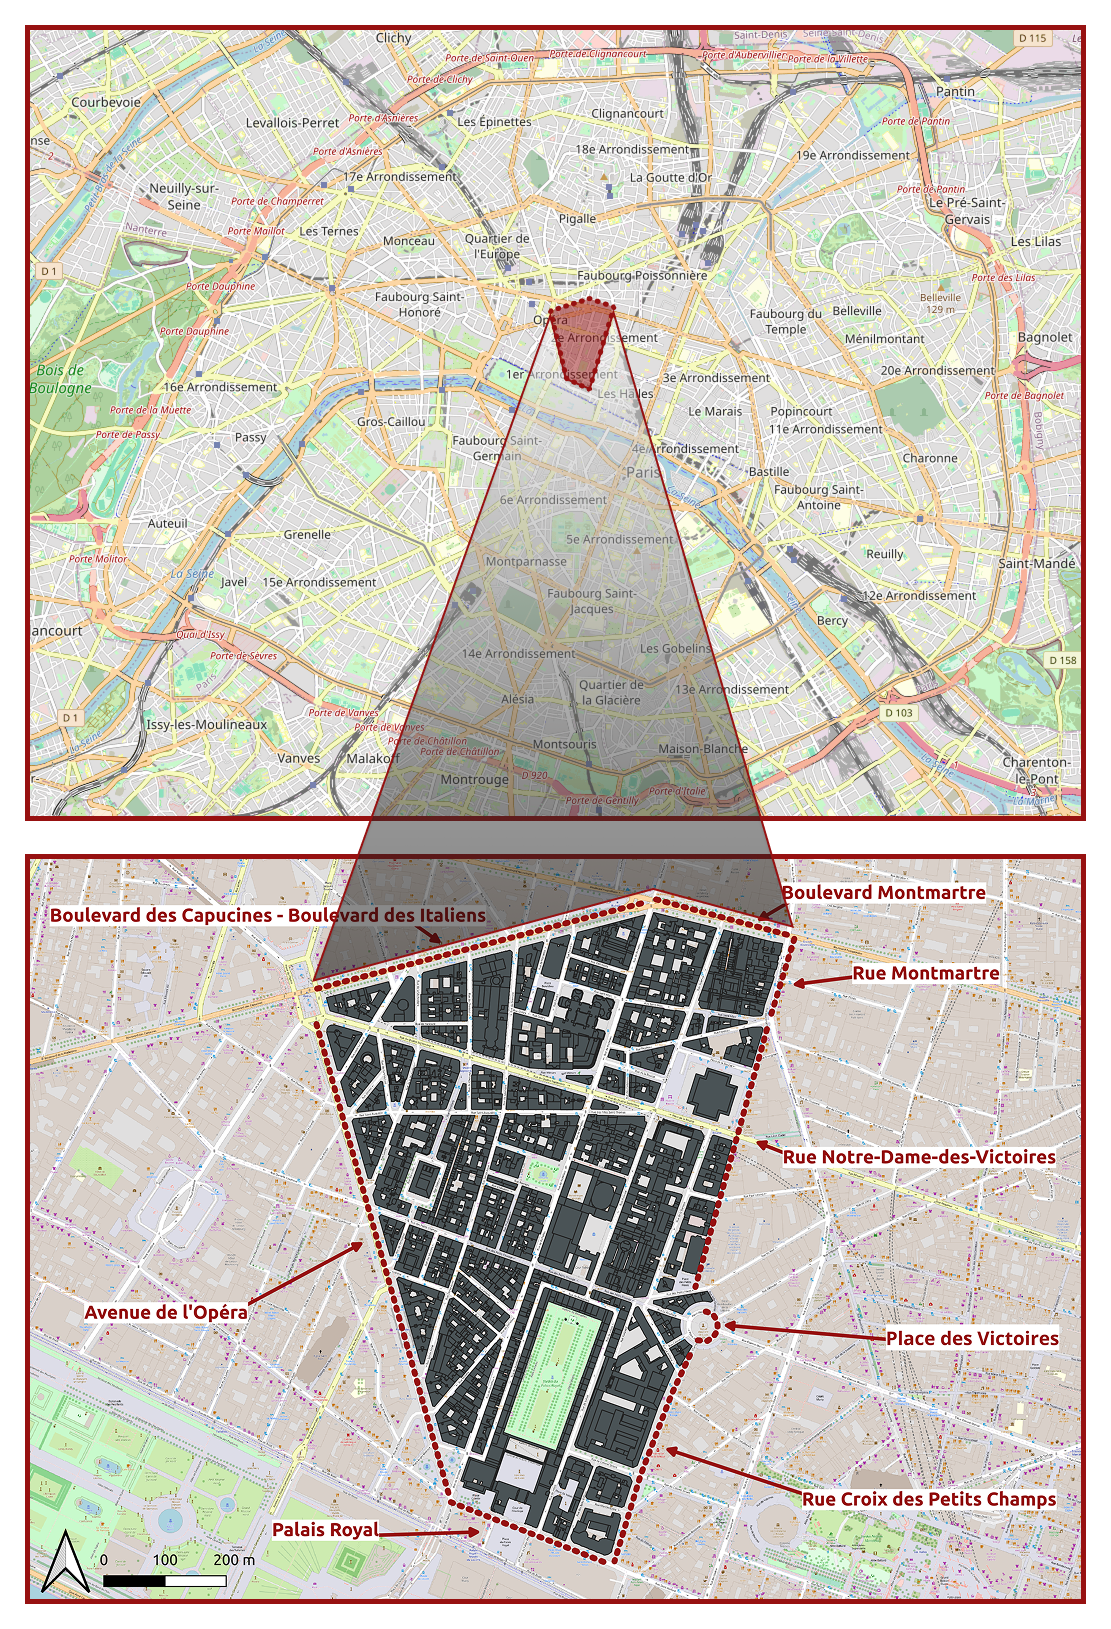
\includegraphics[width=\linewidth]{includes/richelieu_outline.png}
    \caption{Position of the \textit{Richelieu} neighbourhood within Paris}
    \label{fig:outline}
\end{figure}

\subsection{The \textit{Richelieu} city section}

The neighbourhood under discussion, which is not officially recognised, extends itself between the first and second districts, from the \textit{Place des Victoires} to the \textit{Avenue de l'Opéra}, and from the \textit{Palais-Royal} to the \textit{Grands Boulevards}. Between these  four distinct urban typologies lies a multitude of locations, events, services, and monuments. Through their shared history, they collectively shape Paris as a cultural capital \parencite{charleParisCapitalesXIXe2021}. These spaces are interconnected by material and immaterial networks and a shared urban and architectural practice, as revealed through visual sources.

Given the neighbourhood's small geographic scale, an exhaustive research was  conducted through collections of iconographic documents available in the digital databases of public institutions concerned with Paris' history\footnote{
    Amongst the most important data sources for our research are the databases of \href{https://www.parismuseescollections.paris.fr}{Paris Musées}, \href{https://bibliotheques-specialisees.paris.fr}{Bibliothèques spécialisées de la ville de Paris}, \href{https://gallica.bnf.fr}{Bibliothèque nationale de France} and \href{https://www.britishmuseum.org/collection}{British museum}.
}. A granular study was then undertaken, on the micro-scale of a restricted urban area, but whose richness and variety is nevertheless representative of larger trends in urban evolutions. The primary focus of this study is the north-south axis linking the \textit{Palais-Royal}, the \textit{Bourse}, and the \textit{Rue Vivienne}, encompassing the block occupied by the French national bank headquarters between the \textit{Rue Croix-des-Petits-Champs} and the \textit{Rue de Valois}. 

The area in question is notable for its concentration of political and economic power, due to its central position in Paris. It is also a business neighbourhood, with retail shops developing quickly in commercial galleries. Furthermore, it is a popular entertainment district, boasting theatres, restaurants and cafés. The contemporary transformation of urban infrastructure and transportation systems, which are expanding at a rate commensurate with commercial developments, is evident at the local level, in conjunction with overarching trends. These elements collectively influence the evolution of the urban fabric and the behaviours of its denizens, pedestrians, and consumers. The objective of this study is to present a new perspective on this particular example of the European hypercentre, derived from the images it generates and the multifarious interpretations that ensue. The scientific analysis and digital developments have been based on these images, which are the cornerstone of the project.

\subsection{From the iconographic corpus}

This corpus of images, characterised by its heterogeneity, has been produced through a systematic search of street names, monuments, events, institutions and businesses in the digital librairies of several public institutions.

Our extensive collection includes drawings, photographs, trade tokens, business cards, advertising posters, etc. These images not only serve as documentary evidence but also help sketch the early development of a mass culture. In the words of Nancy Steiber, ``The representation of the nineteenth-century city in painting, printmaking, and photography has attracted the attention of art historians and historians of popular culture'' \parencite[388]{stieberMicrohistoryModernCity1999}. In accordance with the sociologist Howard Saul Becker's work these images function as both objects and subjects of study, thereby bearing witness to the collaborative nature of the creation of the city and its images. These images are the product of diverse observational methodologies, through a range of media \parencite{craryTechniquesObserverVision2005}. In some cases, they do not depict the physical space, but rather symbolize the production resulting from human activity in a given location\footnote{
    Our understanding of location and its role in iconographic analysis is further presented in \parencite{kerveganMarqueLieuDans2023}.
}. Through their lens, the images inform the materiality of the spaces they depict as much as the ways in which these spaces were seen by those who chose to represent them. This establishes a link between source and space at a (more or less) given time, whereby space is seen through the filters of the artistic license permitted by each medium. Analyzing this link is an important step towards a better understanding of said space, alongside the diversity of representations that have accompanied it through time. These representations occasionally linger on long after the object of their memory has materially disappeared, shaping our modern understandings of the spaces we inhabit. Thus, our data enrichment method is situated within the interdisciplinary framework of the ``spatial turn'' (\cite{85d83bc2eded406fa8e31f427290f816}, \cite{besse_approches_2010}). In line with this theory, places and their images are regarded as key interpretive tools to understand human, social, and cultural production, as well as how individuals experience and engage with urban and built space.

This phenomenon is evident in the press images published by local media, as well as in the menus offered by restaurants located along these streets. Direct and indirect representations of public space intersect and intertwine, revealing a complex network of connections. This network is essential for understanding the social, urban, architectural, and cultural history of the space -- both as it was conceived and as it is experienced and perceived. The intricacies of this corpus, combined with the multidisciplinary nature of the study, necessitate a qualitative approach to the data, based on localization, enrichment and cross-referencing each image. 

\subsection{... to a digital ecosystem}

The Richelieu Web platform is the conclusion of a complete data management pipeline which encompasses data production, modeling, processing and migration into a robust database. The final step is  the development of a Web platform to showcase the project's data, research and results. As we will see below, this platform also functions as a tool to encourage data reuse, and serves as a ``corpora factor''. This pipeline relies on a complete ecosystem of open-source tools developed specifically for the project. Its aim is to convert research data into \ac{fair}, standards-compliant and reusable data. More than a simple processing or migration of data, the pipeline functions as a translation process of three corpora which constitute the core concepts of the project's database. 

First, the  iconographic corpus consists of 4217 documents, described in an XLSX spreadsheet containing metadata on each of them. It includes standard fields (author, production date, title, URLs linking to the document's location in the digital library where it was found, URL link to the document's \acs{iiif}\footnote{\acl{iiif}} manifest). as well as custom metadata fields created specifically for the project including themes, named entities and places related to each document, as well as a field indicating if the document was produced in the neighbourhood or if it represents it. Indeed, to be included in our database, a document must either have been produced within the neighbourhood or represent it.

A second corpus focuses on cartography and is divided into two inputs. The cartographic corpus describes 495 plots within the neighbourhood across  different historical sources, specifically cadastral surveys conducted throughout the 19\textsuperscript{th} century, and a contemporary OpenStreetMap survey. This corpus is stored in a \ac{gis}, described below. As different historical sources can represent the same plot, those plots are grouped in a  collection of 331 unique locations, stored in an XLSX document. Each location is given an identifier and is mapped to addresses extracted from historical sources.

A last dataset consists of 4 million directory entries that record economic activities in the neighbourhood between 1839 and 1932 \parencite{dilenardoRepopulatingParisMassive2019}\footnote{The production of this source was supervised by Isabella di Lenardo during a first phase of the Richelieu project (2018-2019).}. Due to the dataset's size and the need for further refinement, it has not yet been integrated to the Richelieu database at the time of writing this article.

\section{Enrichment and characterization of a diverse iconography and cartography}

Iconography is the project's cornerstone. The analysis and enhancement of images are central to our approach in understanding the neighborhood. In accordance with the research themes of the project and the polysemy of the sources, we opted for a multifactorial characterization of the iconographic data.

With the aim of locating the information preserved in these images, a cartographic research process was first undertaken. The cartographic corpus includes plans of the district, cadastres, censives\footnote{
    What we refer to as censives of the Ancien Régime are maps depicting censives, meaning land owned by a lord or an institution, on which they collect rents or dues \parencite{braultCartographieCensivesParisiennes2008}.
} of the \textit{Ancien Régime} (17\textsuperscript{th} and 18\textsuperscript{th} century), plot plans, and projects  for building openings dating from the 18\textsuperscript{th} to the early 20\textsuperscript{th} century. Identifiers are assigned to each location (for example \textit{RV1}, \textit{RV2} etc., for each location in the \textit{Rue Vivienne}). These are used to connect iconographic sources to one or more locations. As a result, the places of production, as well as the places represented or linked to the sale of identifiable products and services, are connected to their corresponding iconographic representations. This method reveals the existence of numerous professional and interpersonal networks. In this way, the images, the spaces they depict and their place of production can be understood together, facilitating both diachronic and synchronic readings.

Most of the sources are therefore multi-located. This is particularly the case for the document titled \textit{Paris industriel et historique} (fig. \ref{fig:paris-industriel}), which illustrates and spatializes a selection of the neighbourhood's shops  around 1840. This document is more complex than it seems, as it combines several modes of representation: its central section is a map, which cannot be understood without its promotional aspect. We chose to emphasize the latter by focusing on  the series of advertising panels that frame it. The 21 shop signs are located in the neighbourhood and mapped to the plots present in our cartographic corpus.

\begin{figure}
    \centering
    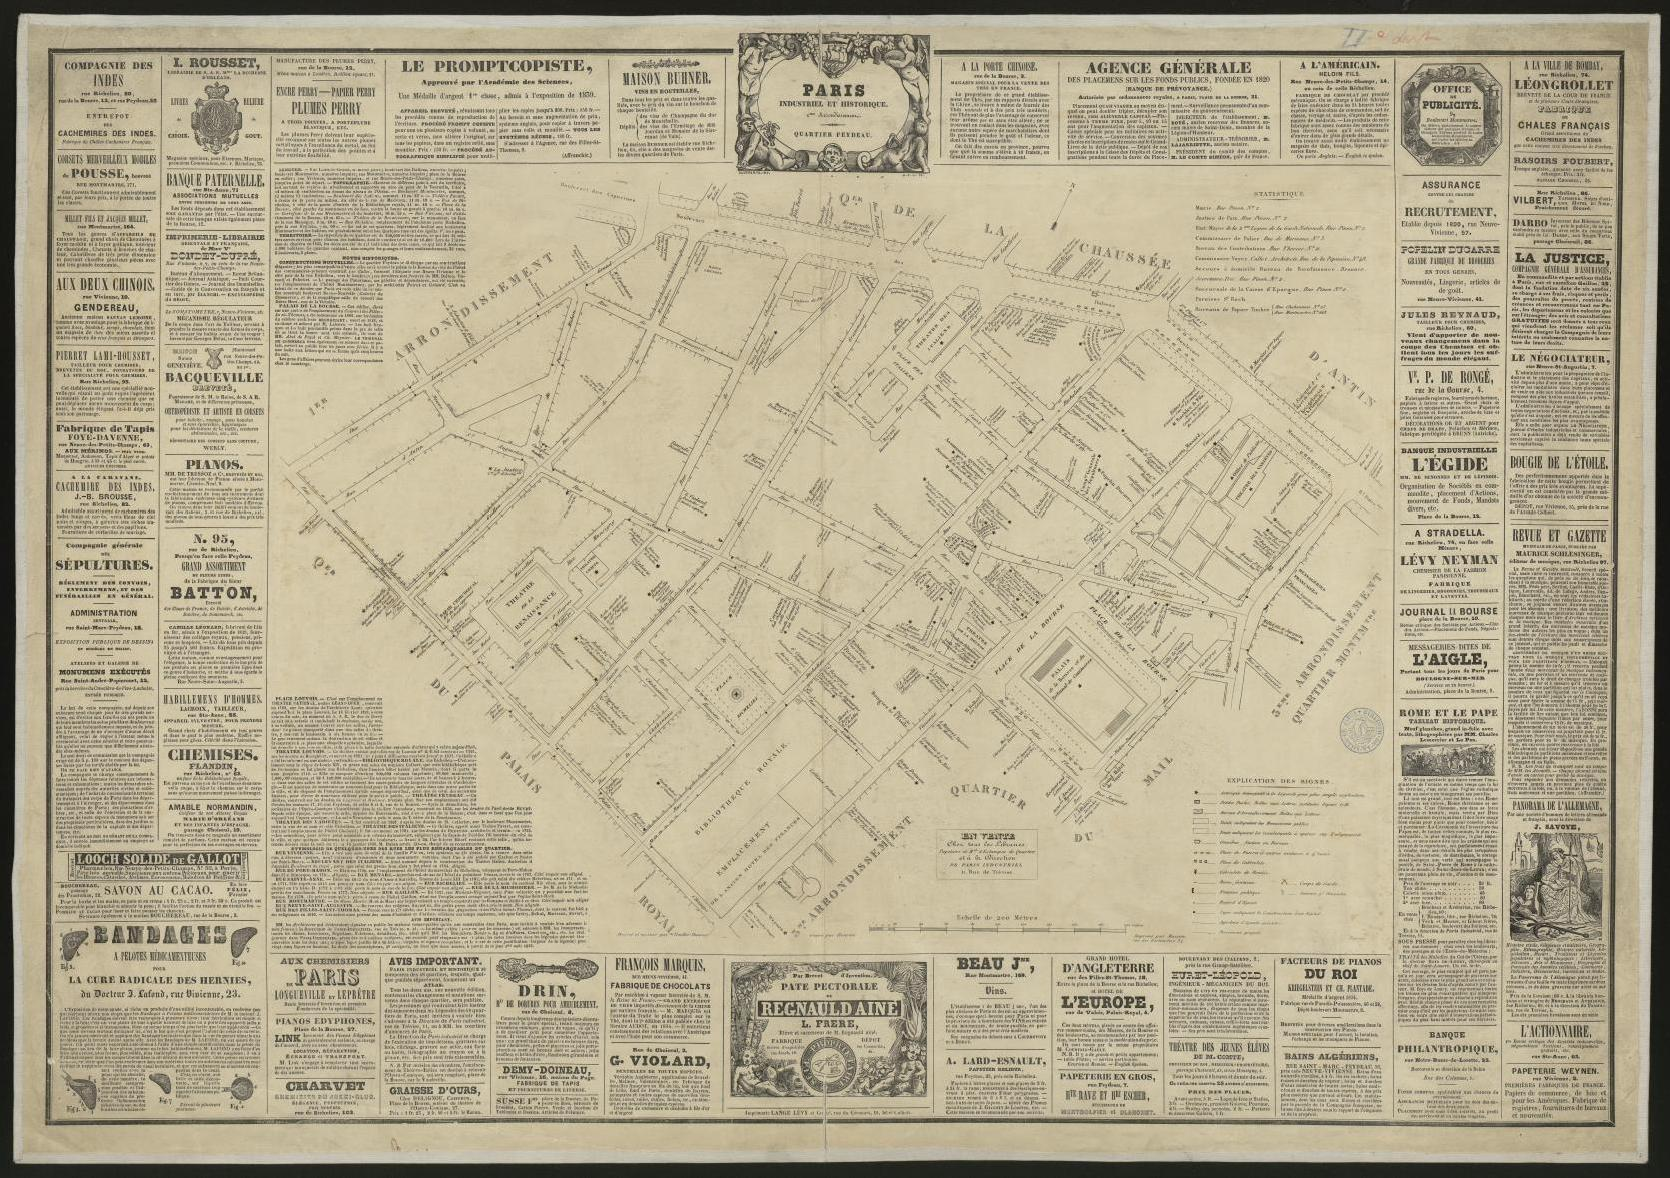
\includegraphics[width=\linewidth]{includes/paris_industriel.jpg}
    \caption{Feuillet-Dumas (drawer), Henriot (engraver), Masson (printer), \textit{Paris industriel et historique. 2\textsuperscript{ème} arrondissement. Quartier Feydeau}, c. 1840, Bibliothèque historique de la ville de Paris, Gr. B7\protect\footnotemark}
    \label{fig:paris-industriel}
\end{figure}

\footnotetext{URL: \url{https://bibliotheques-specialisees.paris.fr/ark:/73873/pf0000853934} (on the \textit{Bibliothèque historique}'s portal) and \url{https://quartier-richelieu.inha.fr/iconographie/qr19ab4064b8fb0403b825a0552aa66fd6f} (in the \textit{Richelieu} platform).}

Through  this example, we observe another data enrichment process, which involves categorizing the sources based on a list of themes and named entities. 60 themes  are  grouped in 6 broad categories defined according to our  research axes and to the initial results obtained (table \ref{table:theme}). The granular analysis of the information conveyed by each image then led to the definition of a similar list of 1118 named entities, grouped within 13 categories (table \ref{table:named_entity}). These specific and highly varied named entities were identified through iconographic analysis and organized within these categories. As far as possible, each document is then categorized into themes, such as `architecture', `public space', and `commerce'; named entities are also identified. Amongst these are clothing stores (e.g., `Popelin Ducarre nouveautés'), the Stock Exchange Palace (`Palais Brongniart'), or objects related to events from the French Revolution (e.g., `Arbre de la Liberté'). These images are linked to our spatialized digital cartography, offering a comprehensive view of the neighborhood's historical and cultural landscape.

These collections  are specific to the neighborhood, as they arise from  the analysis phase of the iconographic sources. Some research axes that were not initially considered emerged during this process, among which is the representations of public space in social and political caricatures from the second half of the 19\textsuperscript{th} century. Certain monuments deeply embedded in collective consciousness seem to have been used by artists as background elements to reinforce their critique of the excesses of capitalism, such as the \textit{Palais Brongniart}, the seat of the Stock Exchange and finance In Jean Veber's caricature (fig. \ref{fig:bourse}), the columns and steps of the Stock Exchange are well visible. Thanks to this spatial information, the document can be connected to the location of the \textit{Palais Brongniart}, and belongs in a sub-corpus of 283 images representing the monument. The document is connected to the following themes: ``press,'' ``current events,'' ``architecture,'' ``caricature,'' and `money'. Through this analysis, we gain insight into public perception, societal attitudes, and the artistic imaginings of the city.

\begin{figure}[t]
    \centering
    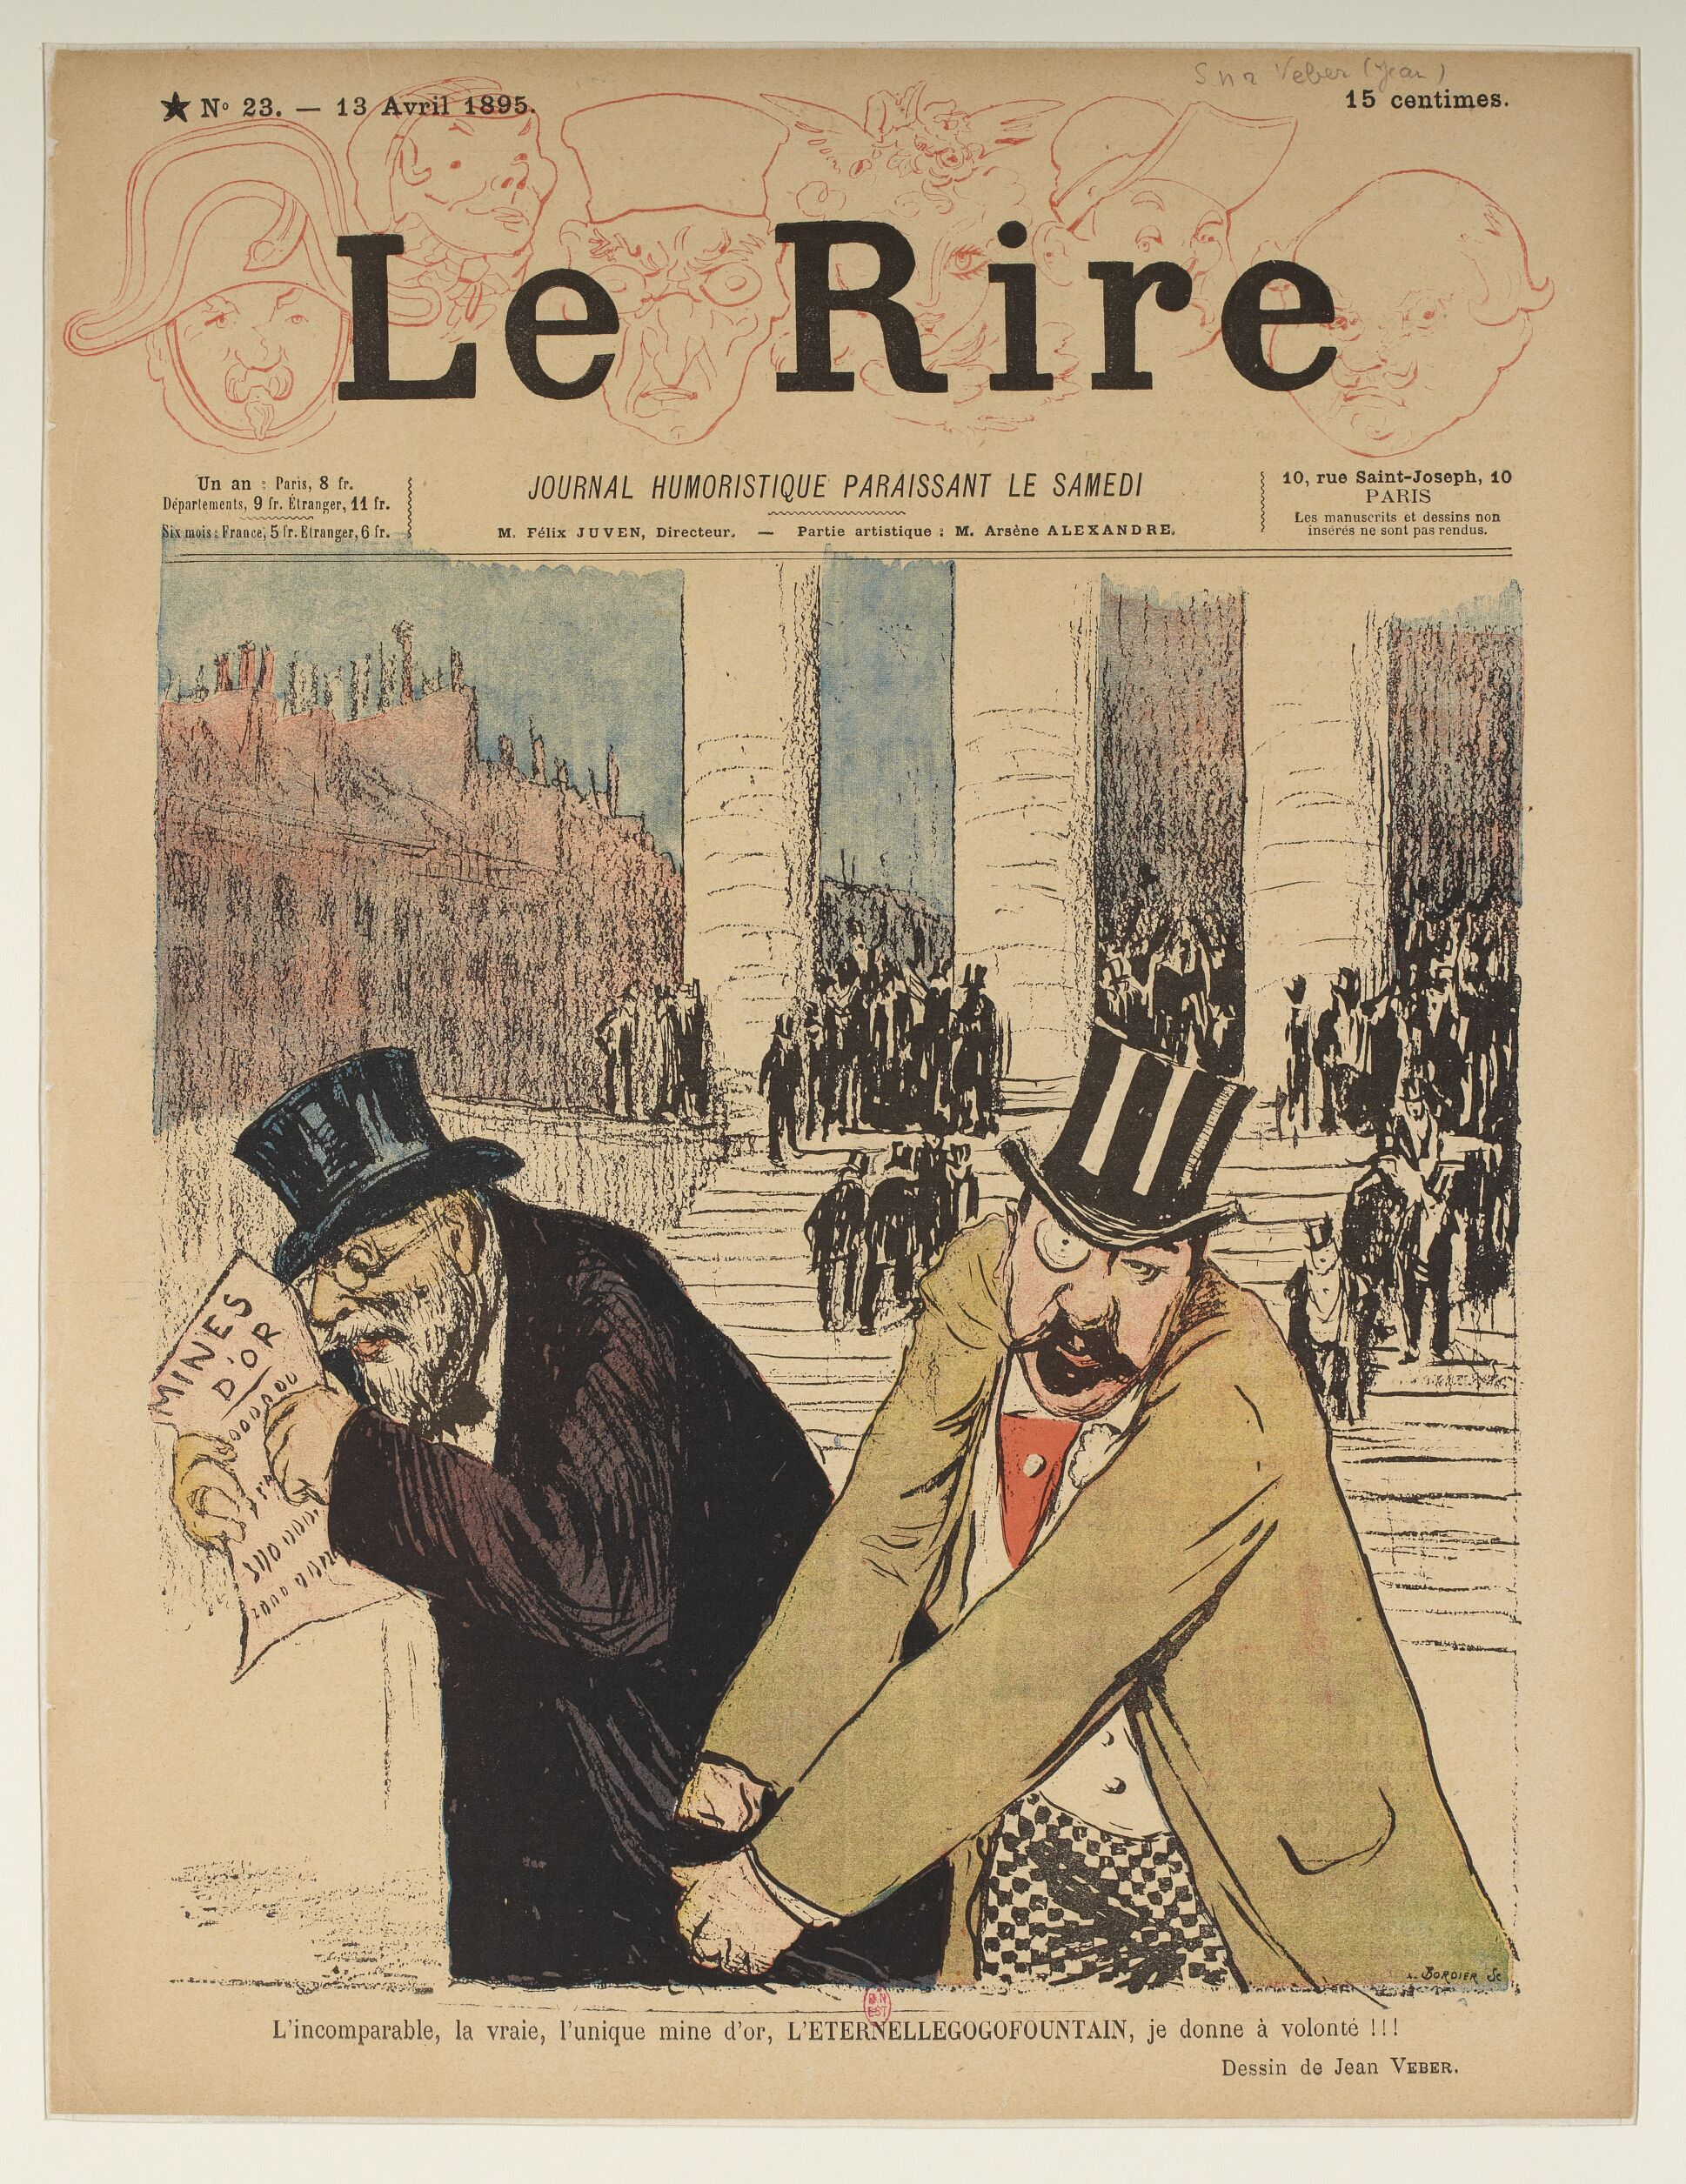
\includegraphics[width=\linewidth]{includes/bourse.jpg}
    \caption{Jean Veber, \textit{L'Incomparable, la vraie, l'unique mine d'or, L'ETERNELLEGOGOFOUNTAIN [sic], je donne à volonté !!!}, 1895, Bibliothèque nationale de France, FOL-EF-490\protect\footnotemark}
    \label{fig:bourse}
\end{figure}

\footnotetext{URL: \url{https://gallica.bnf.fr/ark:/12148/btv1b85775375} (Bibliothèque nationale de France), \url{https://quartier-richelieu.inha.fr/iconographie/qr11d7ee97b99274e20b958eb2866cdde35} (\textit{Richelieu} platform).}

The identification of demolished buildings in the sources has enabled the creation of specific named entities, such as the ``Théâtre des Nouveautés'' (later renamed Vaudeville Theater), inaugurated in 1827 and demolished in 1869 (fig. \ref{fig:theatre}). The 232 ressources linked to this named entity  represent the theatrical and social activities it welcomed. Storez's representation (cited above) also showcases the theme  `public amenities',  (here, railings around the Stock Exchange). This theme is associated to 662 documents in our database. Thus, complex relationships between images, concepts, practices and the build environment emerge from iconographic analysis. In order to systematize this graph-like cross referencing, it is necessary to formalize these relations within a multimodal information system.

\begin{figure}[t]
    \centering
    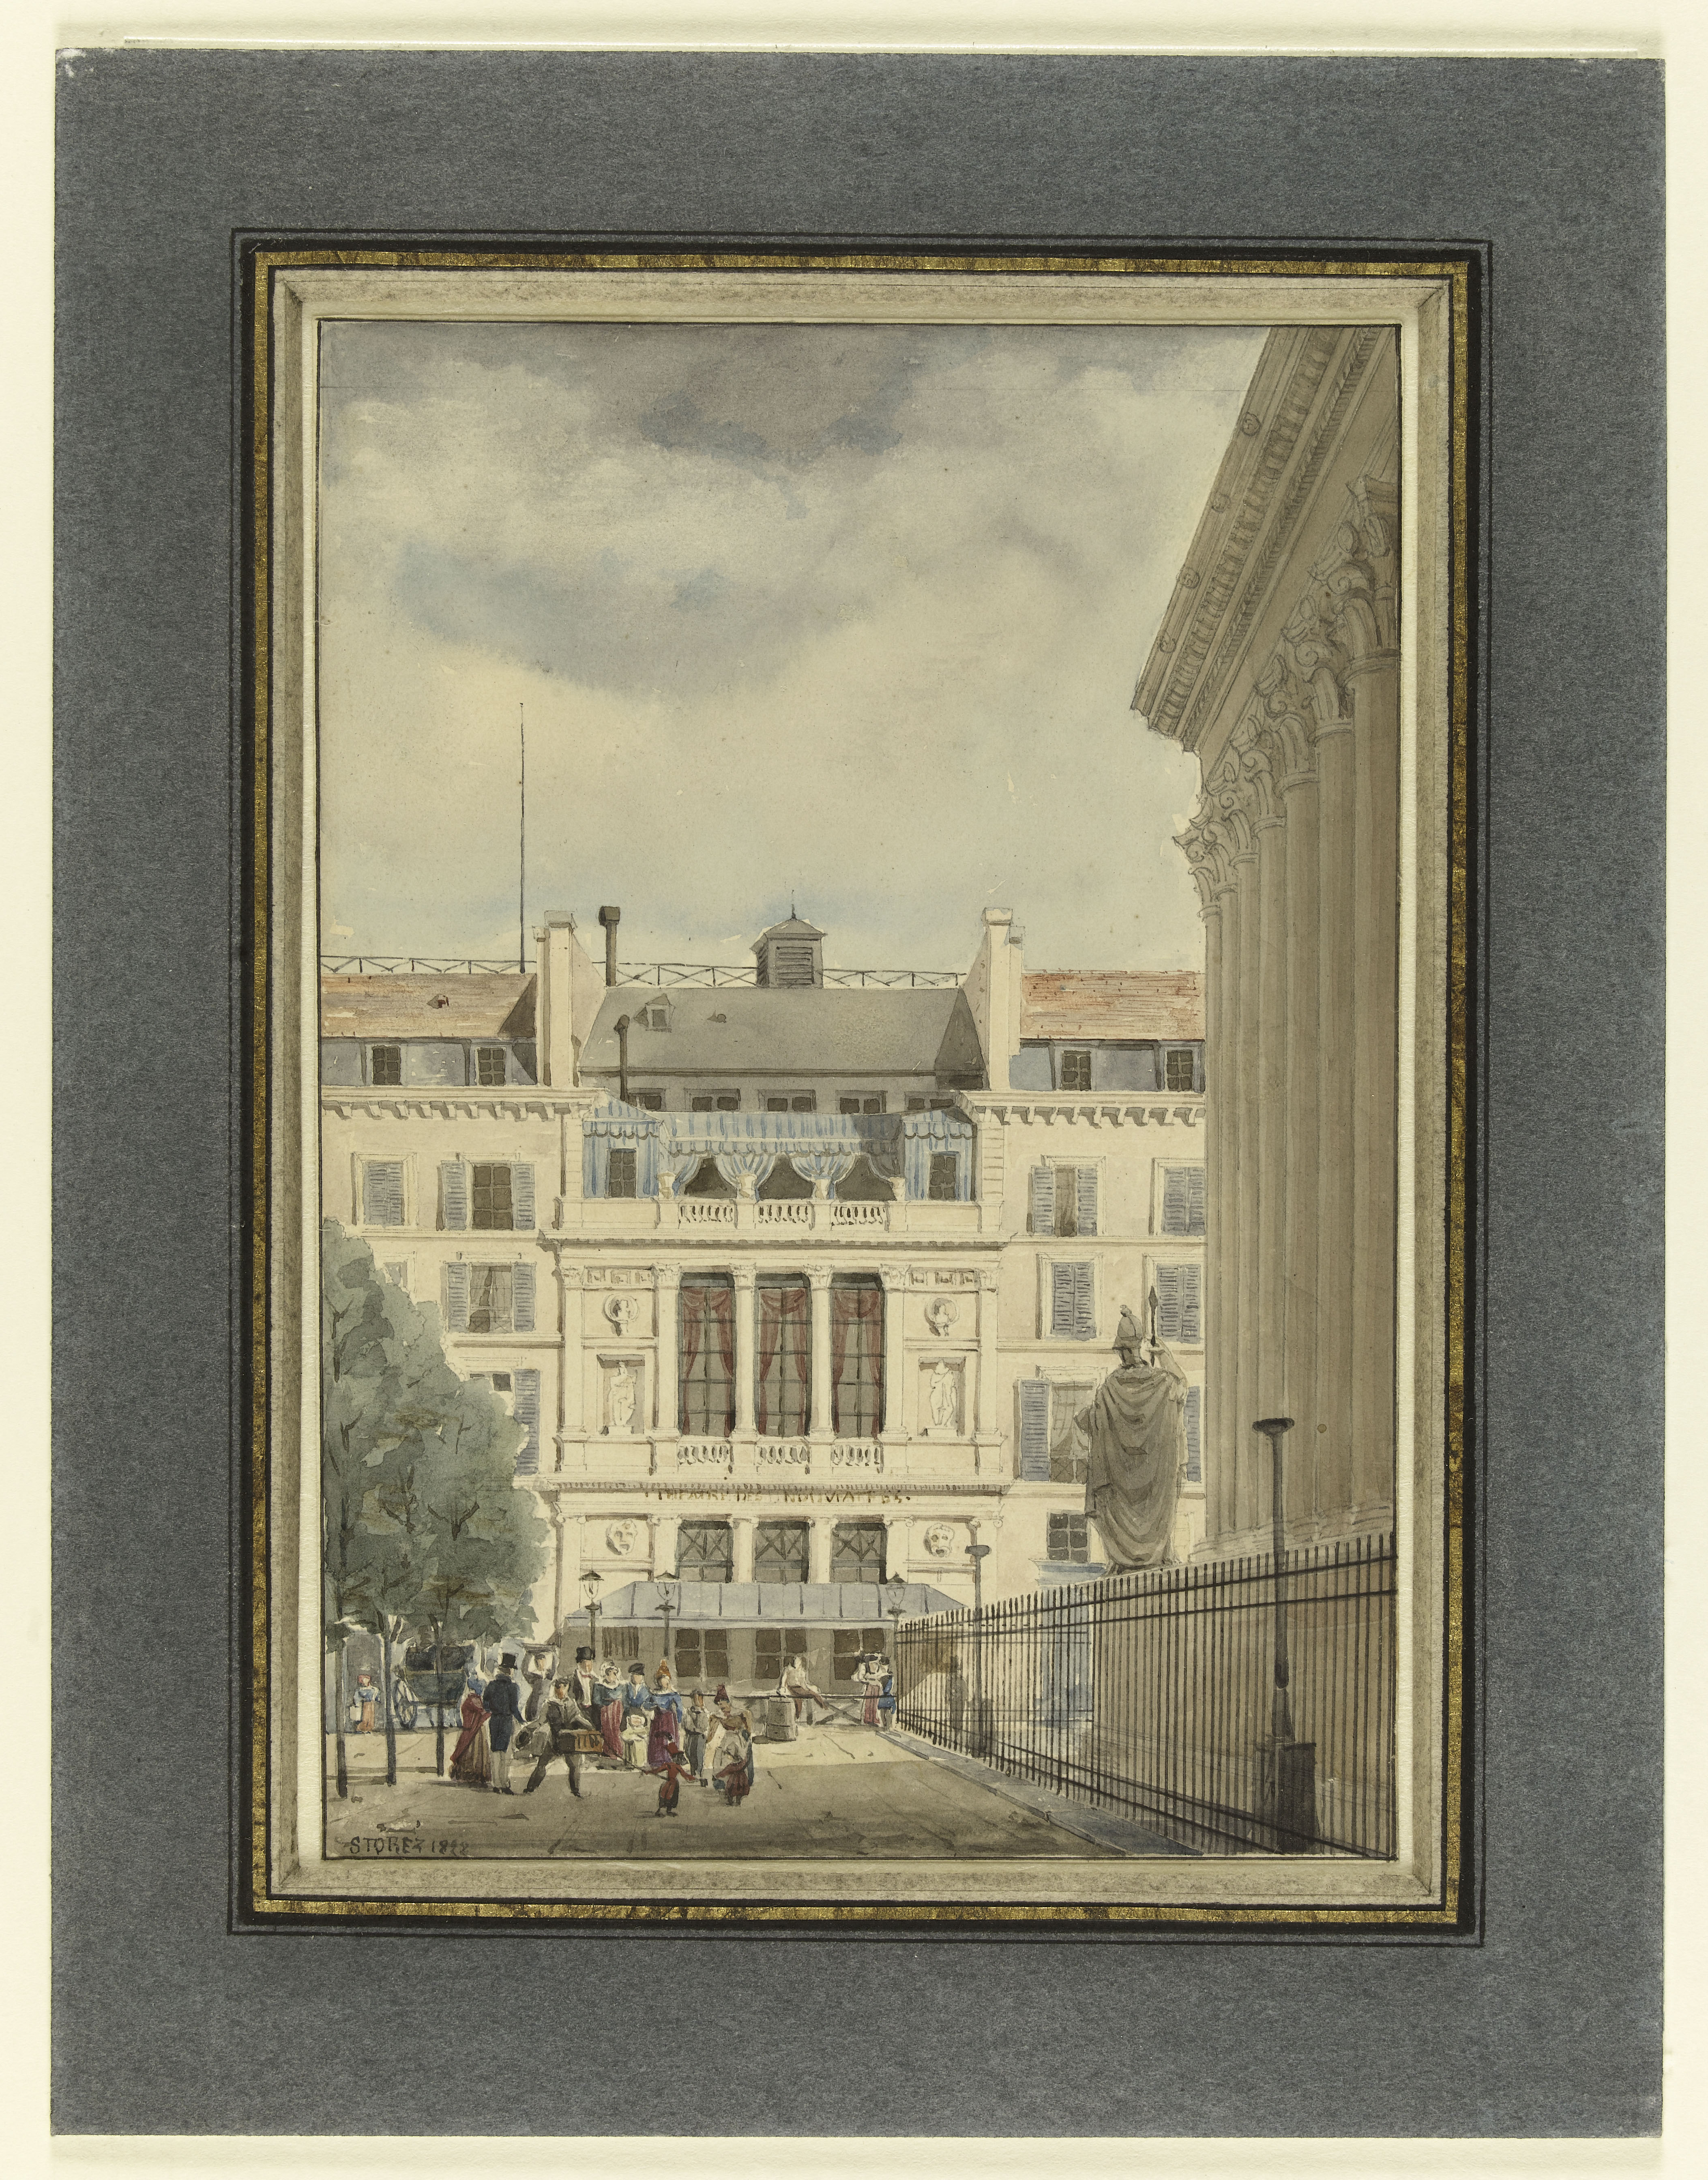
\includegraphics[width=\linewidth]{includes/theatre.jpg}
    \caption{Storez, \textit{Le théâtre des nouveautés en 1828}, 1828, Musée Carnavalet, D.15631\protect\footnotemark}
    \label{fig:theatre}
\end{figure}

\footnotetext{
    URL: \url{https://www.parismuseescollections.paris.fr/fr/musee-carnavalet/oeuvres/le-theatre-des-nouveautes-en-1828} (Paris Musées), \url{https://quartier-richelieu.inha.fr/iconographie/qr1d938f1e4dcf04987828d230ed99674d2} (\textit{Richelieu} platform).
}

A historical \ac{gis} has been developed to spatialize these sources. To create the \ac{gis}, we selected three main cartographic documents who provide an insight into the evolution of the neighbourhood's built environment throughout the 19\textsuperscript{th} century:
\begin{itemize}
    \item the Vasserot cadastral plan (1810-1836, \cite{souchonPhilibertVasserot177318402008}, \cite{noizet:halshs-00419684})\footnote{We reuse a georeferencing carried out by the Alpage ANR project \parencite{costaAtlasVasserot181018362023}.}
    \item the parcelles à la feuille (1809-1854, a corpus stored by the Archives nationales).
    \item the Paris municipal plot plan (1871-1896, \cite{dumasRepresentationDescriptionProprietes1999} \cite{balPlanParcellaireVille2000})\footnote{We reuse a georeferencing conducted by the Paris Time Machine \parencite{costaPlan1900Draps2023}.}.
\end{itemize}

Raster files of each source are georeferenced within the \ac{gis}. Then, these sources are vectorized to obtain a polygon for each plot in the neighbourhood. A location identifier is given to each polygon; the same building will have a unique location identifier across all sources. A raster file is exported for each polygon thus obtained in GeoTiff. Finally, the polygons are exported in shapefiles\footnote{A more detailed presentation of the \ac{gis} is out of the scope of this article.}.

\section{Towards openness: the Richelieu digital ecosystem}

Our data processing pipeline aims to transform the sources presented above into machine readable and actionable data to be presented in a Web platform. Formalizing this pipeline (fig. \ref{fig:pipeline}) is a twofold process: in order to systematize the access to the products of iconographic analysis, it limits complexity and restricts the narratives that can emerge from our corpora. Within this process, data modeling is central. We consider modeling to be an interpretation of data sources, pre-determined by scientific questions and academic conventions. In turn, it determines a set of possibilities, and most importantly limits possible readings of our sources. As Spergberg-McQueen \parencite[288]{sperberg-mcqueenPlayingKeeps2019} puts it, beyond utilitarian needs, modeling can serve ``to capture as completely as possible our current understanding of the thing being modeled''. In turn, we consider that the digital pipeline of the \textit{Richelieu} project functions as a translation, transforming the ``traditional cultural object'' into a ``particular case of a new media object'' \parencite[87]{manovichDatabaseSymbolicForm1999}. After presenting the ``conceptual shift'' \parencite[7]{flandersShapeDataDigital2019a} between ``humanities data'' and ``\acs{fair} data'', we present the project's model. Finally, we present the \textit{Richelieu. Histoire du quartier} web platform, its architecture as well as our approach to ensure FAIRness in an open science context. 

\begin{figure}[t]
    \centering
    \includegraphics[width=\linewidth]{includes/pipeline_main_eng.png}
    \caption{The Richelieu data processing pipeline}
    \label{fig:pipeline}
\end{figure}

\subsection{FAIRness out of humanities data}

The sources of the project can be understood as humanities research data: ``manually produced'', they are made to be understood by humans, and more specifically, by the project's researchers. They require a familiarity with the project's concepts to be understood. In order to make this data useful to a wider audience, it is necessary to decipher these concepts to ensure reusability. 

More problematic to a DH approach, humanities data is unsystematic \parencite[5]{flandersShapeDataDigital2019a} and contains a lot of implicit relationships between different datasets and in-between datasets. These relationships cannot be actionned by a machine and, as such, they limit the efficiency of a computational approach. Such ``weak links'' have to progressively be transformed into ``hard links'' manually (using a system of foreign keys to create relationships between datasets and computational methods, i.e. fuzzy string matching…).

In technical terms, humanities data is weakly structured, since it's made for human readers: data structures can vary between datasets as well as file formats and field separators. A strict data curation process thus is necessary to ensure consistency. 

In their original form, these data sources function in silos. They were produced by researchers from different academic backgrounds (art and architectural history, social and economical history, digital humanities, geography) considering the same research object from different perspectives. For example, a geographer may georeference a map in our GIS, while an art historian will add an iconographic document to our database. Both map and iconography represent the same object. Without explicitly modeling it, the relationship between documents cannot be mobilized. The main aim of the Richelieu pipeline is to break this silo effect and to encourage an interdisciplinary approach in urban studies by producing computational and \acs{fair} data. In order to be reusable by other researchers, our data should:

\begin{itemize}
    \item Be machine readable and actionnable.
    \item Use open-source formats and standards.
    \item Relationships between concepts and resources should be be made explicit.
    \item A consistent data structure is needed, so that all resources can be made available through the same processes.
\end{itemize}

Thus, migrating from humanities and research data to digital, machine actionable data is both a process of reformatting weakly structured information into strongly structured formats \parencite[5]{kembellec:hal-02306958}, and a process of translation, to ensure that our data can be used by others.

\subsection{The database: a conceptual model}

Informed by Johanna Drücker's concept of interpretative modeling \parencite[103-130]{druckerVisualisationInterpretationModelisante2020a} we consider database modeling to be an intellectual process, and our database to be one of the main scientific outputs of the \textit{Richelieu} project, on par with the production of secondary spatialized sources. Database modeling demanded to prioritize certain aspects of our data, while determining which avenues should not be explored.

Our three corpora divided into four inputs constitute the central objects within our database: place, iconography, cartography and directories. The relationship between these objects has been the main concern during the database modeling process, and a differentiation was made between these main objects and auxiliary, ``attribute objects'' that merely characterize our data sources.  

We rely on the neighbourhood's locations, derived from the GIS, to connect the different corpora together: a map and an iconographic document are connected if they represent the same place. In turn, the modeling of space plays a central role in our approach. We consider that a location is independent from its representations \parencite{kerveganMarqueLieuDans2023}.

\begin{itemize}
    \item A location is defined by its spatial and temporal extents. The spatial extent of a location can vary, but typically, the base unit for all of our locations is the plot, that is, a single building within the neighbourhood. For monuments and covered passages, the extent of locations can vary, from a single shop, to a wing or a full building. The temporal extent is the time frame for which we consider a place to exist -- typically, from the moment when a building is created to its destruction. A location is a synthesis of the different cartographic sources representing it.
    \item A cartographic representation of a location is then defined using a specific source georeferenced within a GIS. Due to its relation to a historical source, the cartographic representation is a snapshot in time of a location's state.
    \item In the same manner, a location can be represented by several iconographic documents, and iconographic documents are all connected to spatial data. This allows to work with a spatialized corpus, documenting where each image was produced (if it was produced in the neighbourhood), as well as the locations that it represents.
\end{itemize}

In database modeling terms, there is a one-to-many relationship from locations to cartography and iconography. For example, there are 495 cartographic representations for 331 locations. This allows to create an inheritance relationship between different iterations of the same plot throughout several historical sources. It is also crucial to cartographic visualizations: it is possible to switch from a diachronic view (centered on locations) to a synchronic view, displaying only locations that exist on a specific historical map.

Developing this modular approach to space is key both to the conceptualization of our resources and to data visualization and analysis. Considering locations as minimal objects that are characterized by other sources makes it possible to combine the very different temporalities that exist within our data. While iconography is continuous (documents are produced constantly throughout the 19\textsuperscript{th} century), cartography is discontinuous (maps are produced at specific dates), and the diachronic view offered by locations allows to programmatically determine the most fitting cartographic source to associate with each image, based on their production date.

On the other hand, certain aspects were left aside. Although the materiality of our documents is documented in our database, it is not a main focus. Providing quality data for materiality studies would have demanded an in-depth study that is out of the scope of our research. Prosopographic questions are also auxiliary to our database, although authors and publishers of artworks are documented. This is to shift away from an artist-centric view of art history in favour of a focus on thematic and spatial analysis.

\subsection{Database implementation}

The database uses PostgreSQL, an SQL-based open-source relational database management system. During the modeling process, the use of a graph database was considered, but a relational database was privileged in the end: although graph databases encourage integration within the Semantic Web, the complex modeling required did not fit into the project's time constraints. Moreover, there is relatively limited support for graph databases in Python, the programming language used to develop the website, whereas several libraries provide SQL support. PostgreSQL was privileged for its support of complex types (arrays, JSON and ranges) and because this RDBMS can be extended into a spatial database using PostGIS.

\begin{figure}[t]
    \centering
    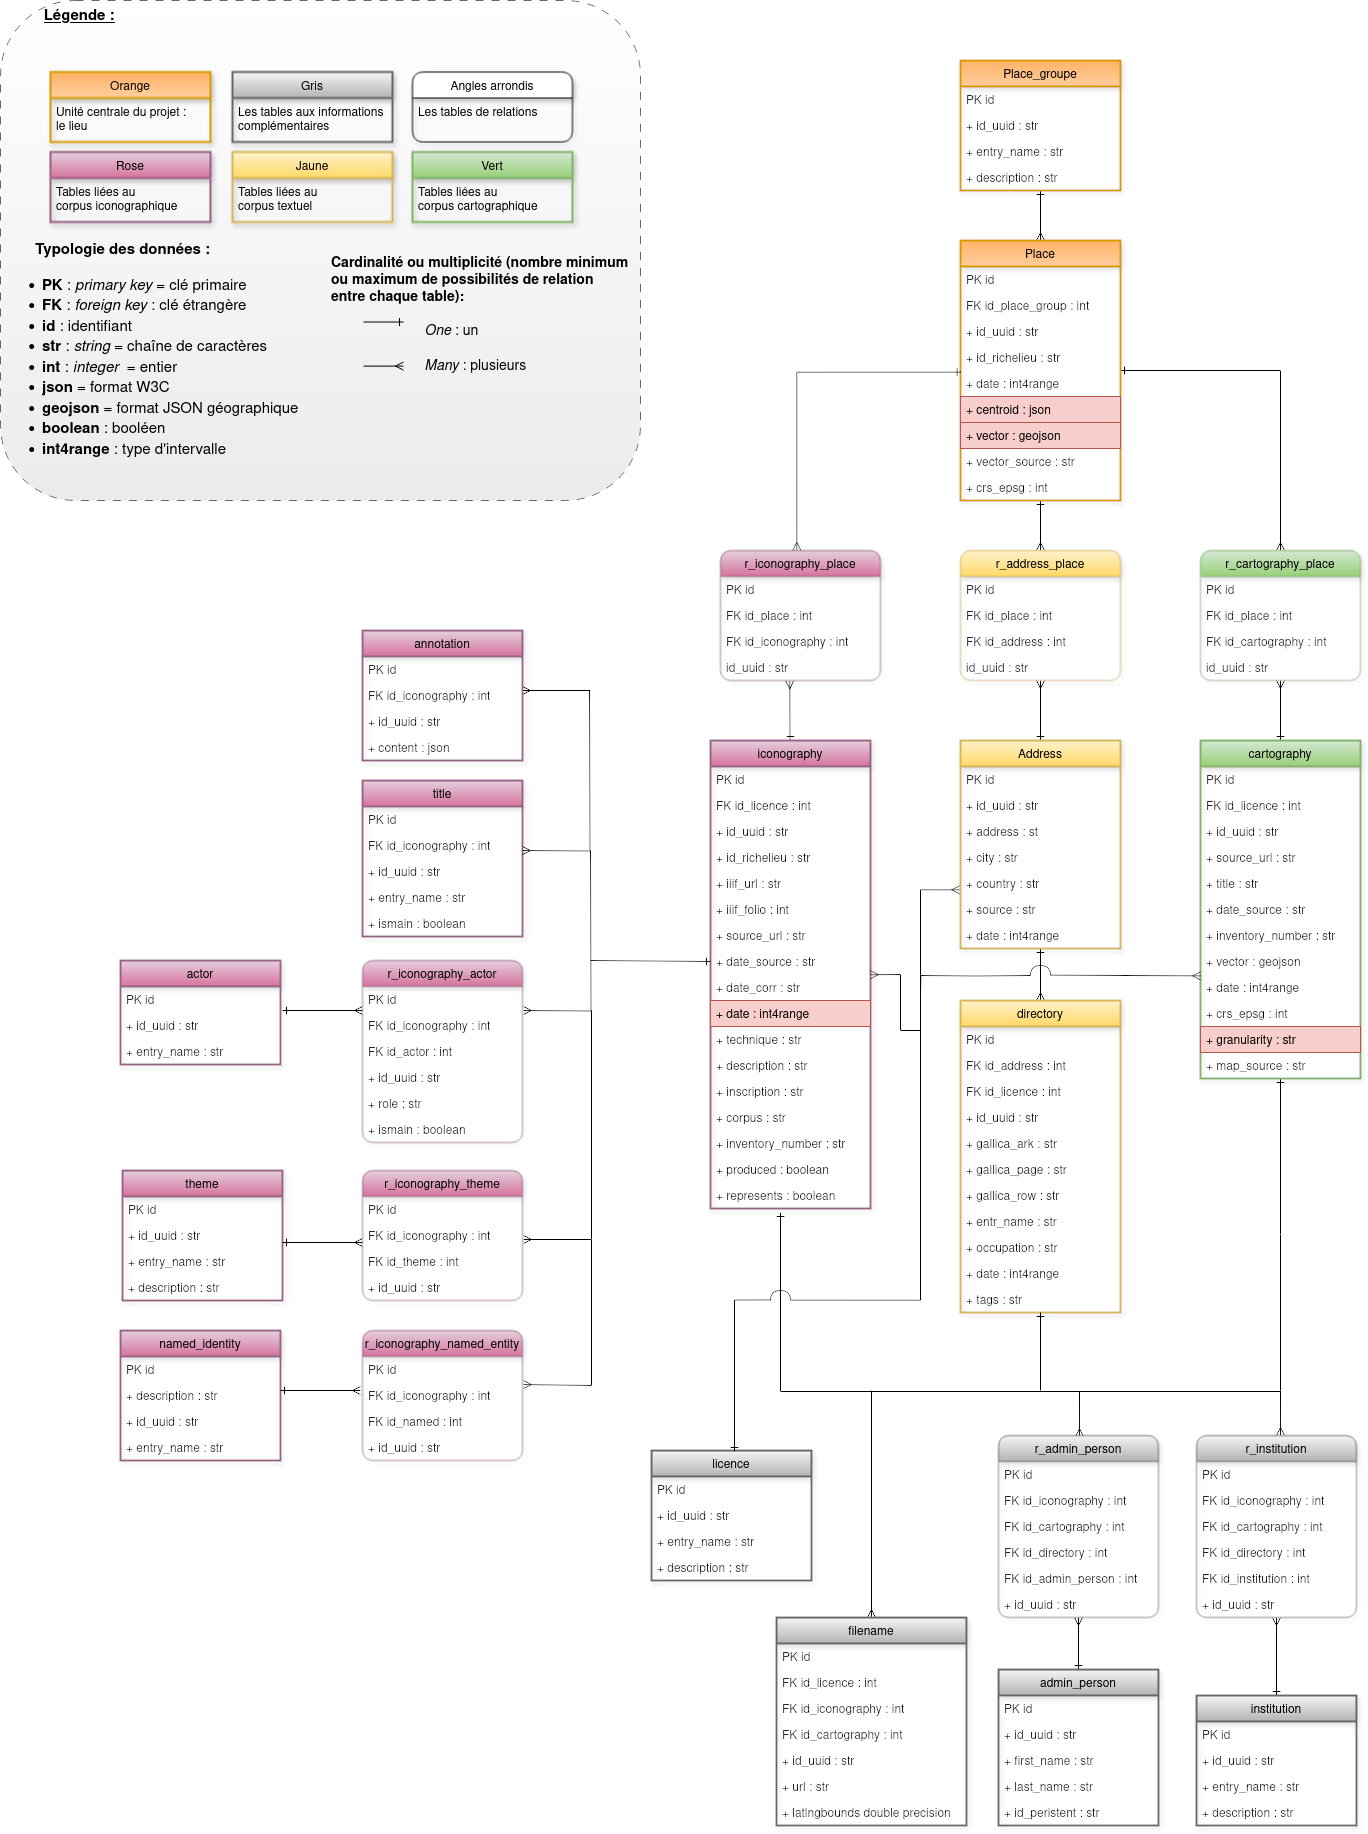
\includegraphics[width=\linewidth]{includes/richelieu_db_model_bg.png}
    \caption{The \textit{Richelieu} database model (credits: \cite[31]{hervieuCartographieWebNouveau2024})}
    \label{fig:model}
\end{figure}

Migration from the four input datasets (iconography, cartography, places and directories) to the database  is done programmatically. During this migration process\footnote{The code for the migration pipeline is stored in the following repositories: \cite{kerveganRichDataData2024}, \cite{kerveganRichDataData2024a}.}, data is simplified and uniformized. Data type conversions are made to fit the database model described above. In some cases, fuzzy string matching is used to cluster variants of a same term in order to normalize notations. Finally, data is reshaped to fit the database's data model. Relationships between the four datasets are made explicit, using SQL's foreign key system\footnote{For an early conceptualization of the role of foreign keys in database modeling and relational algebra, see \cite[379-381]{coddRelationalModelData1970}.}

The database consists of 23 tables (8 relation tables and 15 ``normal'' tables). Given their roles as ways to index the iconographic documents,  themes and named entities are stored in separate tables. Since the database is meant to serve a Web application, technical choices are made to leverage Web technologies. All geographic objects are reprojected to a Pseudo Mercator / WGS:84 coordinate reference system, vector files are converted to GeoJSON, since GeoJSON is natively handled by Python, JavaScript and the Web cartography library Leaflet. As Web support for GeoTIFF is limited, all raster files are converted to standard PNG files, with a bounding box extracted to be able to reposition images within a Web map.

Analyzing the number of relations from themes, named entities and place (later called ``qualifiers'' for brevity) to the ``iconography'' table gives a better insight on the repartition of information within our database (fig \ref{table:graph})\footnote{%
    The code used to produce the analysis is accessible on GitHub: \cite[file \texttt{front/stats\_network.py}]{kerveganRichelieu_jdmdh2025}.%
}. Relationships between qualifiers and iconography can be represented by three directed acyclic graphs: $G_{ne}$ (graph of relations from named entities to iconography), $G_t$ (from themes to iconography) and $G_p$ (from places to iconography). The longest path within each graph is always 1: there is only a direct and one-way relationship from one qualifier to an iconography. In all cases, there is a high disparity in the number of iconographic resources a single qualifier can be connected to. This can be measured by the degree\footnote{%
    The degree of a node is the number of edges it is connected to. In our case, the degree of a named entity node is the number of times it is used to describe the iconography dataset.%
} of each ``qualifier'' node (i.e., each named entity). The minimum degree (noted $\delta$) in each graph is always $1$, while their maximum degree (noted $\Delta$) are: $\Delta(G_t)=1808$, $\Delta(G_{ne})=1088$ and $\Delta(G_p)=875$. In short, a single theme may have between $1$ and $1808$ relations to the iconography dataset. Disparity is brought forward by measuring the outdegree centrality\footnote{%
     In a directed graph, the outdegree centrality of a node $x$ is a measure of its centrality based on the number of edges originating from $x$, expressed as a floating point number between $0$ and $1$.%
} $\delta^+$ of each node in the three graphs. In all cases, the median outdegree centrality is low: $0.00137$ in $G_p$, $0.00189$ in $G_{ne}$ and  $0.042476$ in $G_t$. In $G_ne$ and $G_p$, a very small number of ``qualifier nodes'' are very well connected to iconography: for example, a few named entities are extremely frequently used to qualify the iconography dataset. Opposite to these very central ``qualifier nodes'', most nodes in $G_{ne}$ and $G{p}$ are very rarely used to tag iconography. This is confirmed by extracting mode values\footnote{The mode value is the most frequent value in a sequence.} for all degrees in a graph: for $G_p$ and $G_{ne}$, the mode is $1$: most qualifiers have only $1$ relation to the iconography dataset. Thus, there is a high imbalance between a few places and named entities that are very frequently used, while others appear much more rarely to qualify iconography. Distribution is comparatively more even in themes: the median $\delta^+$ in $G_t$ ($0.042476$) is over 10 times higher than for $G_p$ and $G_{ne}$; the mode degrees for $G_t$ are $(4, 14, 24, 185, 291, 535)$, also indicating a network much less concentrated on a few central nodes. This is partially explained by the small number of themes ($60$, as opposed to $331$ places and $1118$ named entities). This observation is consistent with the way iconographic data has been enriched. Themes were designed in a cross-cutting manner to create broad categories that encompass a large number of images. In contrast, named entities correspond to more specific subjects, individually extracted from each image, which explains why they intersect much less frequently.

\subsection{The Richelieu Web platform}

While the database provides a formal structuring of the project's central concepts and of their interactions, the href{https://quartier-richelieu.inha.fr}{Richelieu Web platform} was developed as an endpoint to give access to the project's data, through a set of digital tools\footnote{The Web app's code is accessible on GitLab: \cite{kervegan_richelieu_2024}}. It was built with the following aims:

\begin{itemize}
    \item Give a unified access to collections of heritage data from various digital libraries.
    \item Ensure traceability of our digital documents.
    \item Provide tools for access to and reuse of the project's data, in accordance with \acs{fair} principles.
    \item Integrate raw data with historical research, through research articles and cartographic visualizations.
\end{itemize}

In recent years, several platforms have been conceived to host and share digital heritage collections. The first trend is to develop ``data-agnostic'' ecosystems, made to be usable with different types of collections. Notably, Omeka \parencite{Omeka2015} and Heurist \parencite{johnsonHeurist2017} offer a low-code or no-code approach to model a database and develop a Web interface for heritage data. They focus on standards compliance and genericity so as to be used on a variety of sources. 

On the other hand, the project \textit{Richelieu}'s platform is developed ``from scratch'' and tailored specifically to the project's data and scientific discourse. The downside from this ``from scratch'' approach is reusability and adaptability: since the platform uses no CMS, it is necessary to interact with its  code to modify its contents.

For modularity, the platform is twofold:
\begin{itemize}
    \item A backend handles database interaction (querying, retrieving, remodeling data) and provides two APIs -- an internal one, consumed by the frontend, and a public API to share raw data to other users.
    \item The frontend focuses on user interaction; it provides a graphical interface, visualizations etc. 
\end{itemize}

The backend is written using the Python Web framework Flask and the SQLAlchemy library for database interactions, while the frontend relies on Vue, a JavaScript framework. All of these tools are open-source. The two parts communicate through HTTP, via an internal API. 

The Web platform's frontend is divided into four parts.

\begin{enumerate}
    \item A ``collections'' module gives access to the project's data: all \href{https://quartier-richelieu.inha.fr/iconographie}{iconographic resources}, \href{https://quartier-richelieu.inha.fr/lieu}{locations}, \href{https://quartier-richelieu.inha.fr/entite-nommee}{named entities}, \href{https://quartier-richelieu.inha.fr/theme}{themes} and \href{https://quartier-richelieu.inha.fr/institution}{institutions} are accessible. As we have demonstrated above those collections are cross-referenced, and, leveraging our database design, it is for example possible to access iconographic resources related to a named entity, a theme or a location.
    \item An \href{https://quartier-richelieu.inha.fr/recherche}{advanced search module} allows querying iconographic resources with more precision, filtering data by institution, title, theme, dates… Several values can be provided for all fields, and it is possible to change the boolean relations between fields to create complex queries. 
    \item A \href{https://quartier-richelieu.inha.fr/cartographie}{cartographic interface} provides a view of the neighbourhood's geography. It functions as a lightened Web-rendition of the project's GIS. It provides historical map backgrounds ranging from 1791 to 1943, as well as contemporary backgrounds provided by OpenStreetMap. On the map background, the neighbourhood's 331 locations are projected. Each location is defined by a polygon. This interface is interactive. This allows to filter the locations displayed by place, by number of iconographic resources connected to each place, as well as to switch between different cartographic sources. Indeed, by default, the map provides a synchronic, location-centered view: all locations are displayed, so historical sources may be mixed together. Selecting a specific cartographic source will only display locations present on it, offering a diachronic view. Finally, all plots visible in the map can be queried: clicking on a location displays all iconographic resources related to it. Plot interactions are also highlighted: when clicking on a plot, the locations that co-occur most frequently with the selected one are highlighted. This is made possible by the enrichment of iconographic sources and gives a glimpse of the networks of interaction that structure the built environment.
    \item The final module focuses on presenting 14 research articles on the neighbourhood. This has been one of the main focus points during the website's development phase: it was conceived as an editorial project of its own, integrating each article with research data. The layout is made of three sections (fig. \ref{fig:article}): the article itself (a); a \acs{iiif} viewer displaying images central to the article (b); a collection of images related to the article's content (c). Pictograms within the article allow to toggle between the images displayed in the \acs{iiif} viewer; the collection of documents displayed at the bottom is built by running custom queries on the database. This module's data structure connects the article's content to JSON objects storing metadata. This controlled metadata is used to build database queries that populate the \acs{iiif} viewer and collection of related documents. Thus, the articles' data model blends free text with structured data in order to integrate a data-centric approach with humanities research.
\end{enumerate}

\begin{figure}
    \centering
    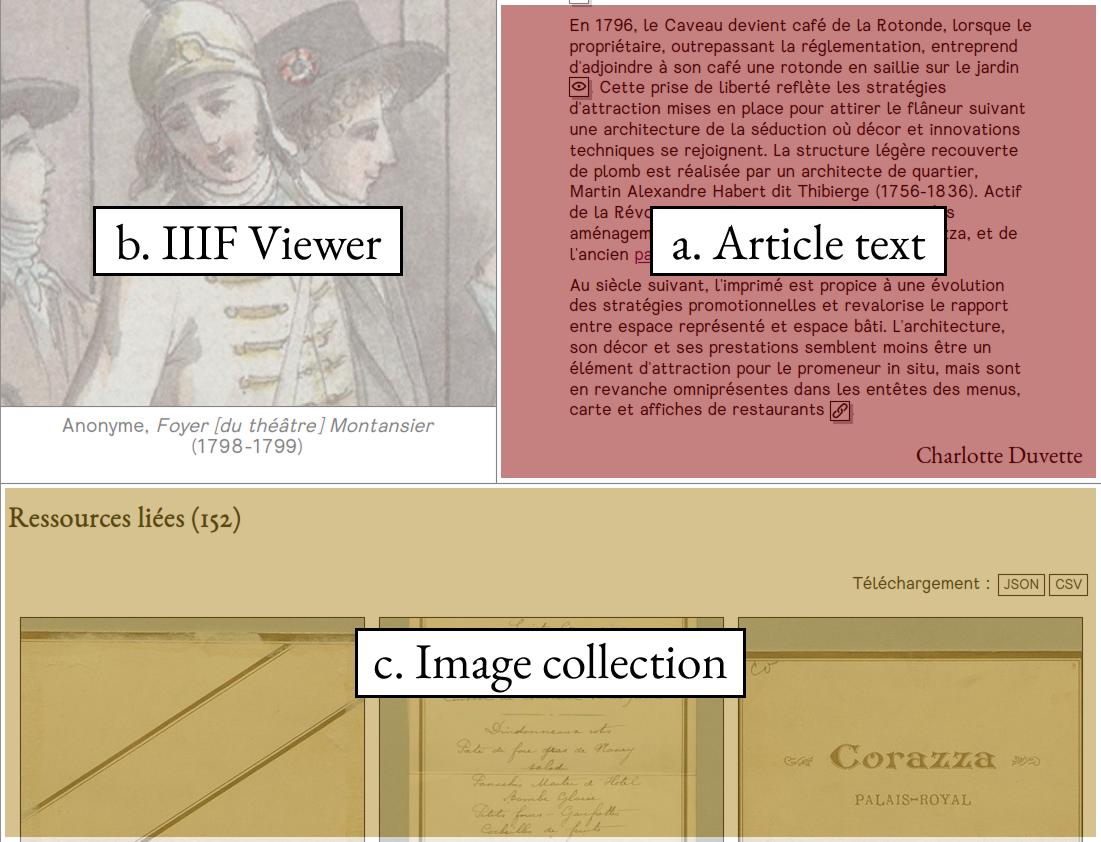
\includegraphics[width=\linewidth]{includes/richelieu_article.png}
    \caption{Structure of the articles on the \textit{Richelieu} platform}
    \label{fig:article}
\end{figure}

\subsection{Open and \acs{fair} data}

Making our data shareable and reusable has been a guiding principle in the development of our platform. Instead of attempting to conform to an abstract definition of what ``\acs{fair} data'' should be, it is important to characterize the data produced by the project, and thus better understand its potential for reusability. Following Kambellec's \parencite[5]{kembellec:hal-02306958} dichotomy between data-as-gnosis and data-as-discovery\footnote{
    Data-as-gnosis characterizes data as the proof of a theory, while data-as-discovery is ``agnostic'' data made to be used as an object of further scientific analysis by others. This dichotomy should be nuanced: data is as much a response to pre-existing questions as it is the starting point for further research.
}, our data could be characterized as ``agnostic'': our wide ranging database provides raw material for future studies. As such, our data should not be shared following the habits of a specific academic culture, but rather be reusable by researchers from a variety of backgrounds. This determines the technologies used for data sharing, but also the structuring and documentation provided to ensure the data is understandable by others. By definition, open data should be reusable, which requires an understanding of who uses the data and of their skillset: data is only reusable insofar as users have the capacity to reuse it. Throughout the project's lifecycle, a wide variety of users have been identified, from institutional partners and heritage institutions, to academics and researchers of varying technical proficiency. Thus, it was not only necessary to share machine-reusable data, but also to make it accessible to non-technical users.

The \acl{iiif} has been the project's technological backbone , and a central tool in ensuring \acs{fair}ness. The widespread use of \acs{iiif} in the heritage and research fields ensured that our data would find its public: indeed, this technology is used by major cultural institutions \parencite{moreux:hal-04675821} and has gained traction among humanities research projects focusing on visual data (\cite{albouy2024aikon}, \cite{hart:hal-04615362}). In the data production phase, we retrieve \acs{iiif} manifests describing documents in our database from research institutions. This ensures traceability, since the manifests act as a hard link between our database entries and online libraries. \acs{iiif} also provides tools to share images and their metadata in standardized, machine actionable formats. Thus, its use is essential in our Web platform: it allows to ship together an image and its metadata, handle single-image documents as well as more complex, multi-image ones, and provide interactive viewing interfaces for very high definition images, using the OpenSeadragon JavaScript library. However, it is necessary for us to store resources accessible through \acs{iiif} as raw image files, both as backups and because external \acs{iiif} servers may block a client after an excessive number of queries. Not all online collections provide \acs{iiif} endpoints, and thus our entire corpora could not be shared through \acs{iiif}; although it is possible to generate \acs{iiif} manifests from our database, implementing a \acs{iiif} server was out of the project's scope.

The Richelieu Web platform provides a REST API \cite[76-106]{fieldingArchitecturalStylesDesign2000} which allows users to query and retrieve information from the entire database in JSON format. It was developed after the platform's internal API that ensures communication between the backend and frontend; the design of both APIs  differs widely. The internal one  is opinionated: its response format is determined by the frontend's needs and relies on a thorough understanding of the database model. The public API, on the other hand, is as ``agnostic'' as possible: it provides three views for each table: a ``catalog'' view listing all entries in the table, a ``light'' view providing detailed information on a single entry of a table and a ``detailed'' view, providing information on a single entry of a table, as well as this entry's relationships to other tables; these are expressed as JSON objects pointing to the routes that should be queried to retrieve data on relationships. This response model makes it possible to query the database in a composable and modular manner. The API's design aims to lower the minimal amount of scientific knowledge necessary to reuse the project's data. Each response has a stable and documented data model specifying its fields and data types. Given that the API's responses follow closely the database's design, the latter's documentation \parencite{kerveganRIchelieuHistoireQuartier2024} should provide the necessary information to understand the API's responses. Thus, the platform's public API provides a way to retrieve the entire database's contents in machine actionable formats, for institutions as well as technically proficient individual researchers.

So far, our discussion on data reusability has left aside the non-technically proficient researchers, as using IIIF and APIs requires some programming knowledge to construct batch HTTP queries and to extract information from JSON responses. In turn, export functionalities were also developed, to download the database's contents from the Richelieu frontend's GUI. Exports are available from the different collection views of the website (institutions, themes…). The contents of an export may vary depending on filters defined by the user through the frontend interface (it is for example possible to filter a collection of iconographic documents based on their date of production or their title). Two export formats are defined: CSV -- a minimally structured and easily usable text format -- and JSON, which provides better structuring. Exports contain the UUIDs of database entries. Using those UUIDs, it is possible to query the platform and its API, thus providing a connection between the different means we provided to access data.

Although we seek to provide reusable data, we are only providing a single access point for it -- the Richelieu platform --, limiting its reusability. Taking \acs{fair}ness a step further would require us to provide data from external platforms. To this end, other avenues have been explored. A next step would be to publish our data on a stable repository (i.e., Nakala), with a companion data paper to describe the production process and scientific choices.

\section{Prospections: a 3D reconstruction of the \textit{place de la Bourse}}

In addition to the four entry points to the neighbourhood's iconography on the project website (cartography, themes, named entities, and articles), a fifth development has been considered: a historical 3D model built using the project's iconography. Indeed, the most well-documented spaces -- presumably those most noticed by contemporaries and indicative of urban, architectural, and socio-economic transformations -- are represented by a heap of images that can be used as raw data in 3D modeling. 3D reconstruction can then be leveraged to study a location's history by layering successive temporal states.  Because historical 3D modeling requires a comparison between archival or artistic documents and the built environment within a 3D space (\cite{aubryPaintingto3DModelAlignment2014}, \cite{aubryPaintingto3DModelAlignment2014}), it can reveal the points of convergence and distortions between the city as it was planned and the city as it is perceived by its contemporaries. This exploratory initiative was proposed based on the project's corpus and is still under development. 

Many of the sources out of the 4217 total are views in perspective, linked to the architectural materiality of the neighbourhood, which is featured both on the forefront and in the background of many a drawing, engraving or photograph. Their concentration is especially important around certain spaces, which has led us to develop a prospective project focused on one such place of interest: the place de la Bourse and its surroundings. The first step in this project is then to select the iconographic documents relative to this space regardless of chronology, that feature at least in part architectural elements or a mention of geography that allows us to locate it in the vicinity of the place.

A first approach for the study of the articulation between space and source is  to move beyond the identification of the source to an address, which involves a relation to time, to an absolute positioning of the source in space. This is  done through a 3-step extension of the Richelieu \acs{gis}\footnote{
    This extension of the \acs{gis} is unique to the 3D modeling process and is not re-integrated within the rest of the pipeline.
}:

\begin{enumerate}
    \item The \acs{gis} is  expanded with a few additional maps allowing for a visualization at finer granularity of the changes that took place between the late 18\textsuperscript{th} century and the mid 1950s'.
    \item The most recent sources are  given an approximate position and orientation in the \acs{gis}, using the identifiable features that could be found in the documents. The sources are  visualized as a standardized cone of vision on the map.
    \item The information obtained about the urban space from this first georeferencing is  used to situate older sources as well as those representing specific details of the place de la Bourse, which feature elements that are not  directly identifiable today.
\end{enumerate}

These three steps thus constitute an iterative process, as every new source integrated into the \acs{gis} sheds a new light on the architectural evolution of the urban space. It might then be necessary either to gather additional cartographic sources to complete the chronology, or  to continue to locate other iconographic sources.

This work of localization has been completed for around 300 different documents ranging from the late 18\textsuperscript{th} to the mid-20\textsuperscript{th} centuries. It notably outlines the variety of ways the sources relate to space, from a caricature's simple evocations of the Bourse to pictures of specific urban elements such as kiosks. The integration of the sources within the \acs{gis} allows for a certain number of analyses to be done on the corpus. Visualizing the collection allows us to notice standard compositions such as the frequent standardized representations centered on the \textit{palais Brongniart} in the first half of the 19\textsuperscript{th} century, the focus on some specific areas prior to and during their destruction during the construction of the \textit{rue de Réaumur}, and the changes in the density and production of iconographic sources brought by the diffusion of photography \parencite{mendibilDispositifFormatPosture2008}.

Photographies have a special place in this corpus due to their method of production: thanks to the optical parameters of the camera there is a mathematical link between the image and the objects it features. Through this relation it is possible to envision a more detailed reconstruction of space through the images produced and of how these images were produced in said space. With about 100 photographs of the \textit{place de la Bourse} and its surroundings, we have explored the possibility of using these documents and this relation to establish a more precise localization in space, eventually allowing for reconstruction.

The process tested out consists of positioning the corpus of photographs relative to a 3D model of the \textit{place de la Bourse}, using the relation linking object and image through the pinhole camera model. This model describes the projection of 3D object space to 2D image space through the optic instrument that constitutes the camera. To parametrize this relation we dispose of several parameters:

\begin{itemize}
    \item Intrinsic parameters relate to the properties of the camera itself: \begin{itemize}
        \item $f_x$ and $f_y$ are the focal lengths of the camera along the two axes of the sensor, but may be distinct for an asymmetrical lens.
        \item $c_x$ and $c_y$ are the position of the image's principal point, i.e. the point of intersection between the optical axis and the sensor.
        $k_1$, $k_2$ and $k_3$ are polynomial coefficients corresponding to lens-induced distortion.
    \end{itemize}
    \item Extrinsic parameters describe the relationship between the camera and the real world: \begin{itemize}
        \item The rotation matrix $R$, containing 9 coefficients that indicate the external orientation of the camera in the global reference frame.
        \item The translation matrix $T$ containing 3 coefficients for the location of the camera in the global frame of reference.
    \end{itemize}
\end{itemize}

The equation that can then be established between an image point expressed in pixels in the image coordinate system and those of an object point expressed in the reference coordinate system is as follows\footnote{
    This equation is based on \cite{majumderCameraCalibration}. 
}: 

\[
\scalemath{0.9}{
    s
    {\underbracket[0.6pt]{
        \vphantom{\begin{bmatrix}.\\.\\.\\.\end{bmatrix}}%
        \begin{bmatrix}%
            u\\v\\1%
        \end{bmatrix}%
    }_{\parbox{1cm}{\centering\tiny 2D image coordinates}}}
    = 
    {\underbracket[0.6pt]{%
        \vphantom{\begin{bmatrix}.\\.\\.\\.\end{bmatrix}}%
        \begin{bmatrix}%
            f_x & 0 & c_x\\%
            0 & f_y & c_y\\%
            0 & 0 & 1\\%
        \end{bmatrix}%
    }_{\parbox{2.5cm}{\centering\tiny Intrinsic parameters}}}
    {\underbracket[0.6pt]{%
        \vphantom{\begin{bmatrix}.\\.\\.\\.\end{bmatrix}}%
        \begin{bmatrix}%
            r_{11} & r_{12} & r_{13} & t_1\\%
            r_{21} & r_{22} & r_{23} & t_2\\%
            r_{31} & r_{32} & r_{33} & t_3\\%
        \end{bmatrix}%
    }_{\parbox{3cm}{\centering\tiny Extrinsic parameters}}}
    {\underbracket[0.6pt]{%
        \vphantom{\begin{bmatrix}.\\.\\.\\.\end{bmatrix}}%
        \begin{bmatrix}%
            X\\Y\\Z\\1%
        \end{bmatrix}%
    }_{\parbox{1cm}{\centering\tiny 3D world coordinates}}}
}
\]

To start with, a lasergrammetric scan of the place is conducted to obtain a precise point cloud\footnote{
    This scan was carried out by the research unit Plemo 3D (Centre André Chastel) for the Richelieu project in 2023.
}, transformed into a lighter model for repositioning the images. This model is then integrated in an open-source modelization software, Blender, where it was given world coordinates through the use of the Blender \acs{gis} plugin.

The repositioning of the images using the 3D model can then be done through the resolution of a system of equations of the form defined above, where the image coordinates and object coordinates are known. Practically, this involves identifying image points on the iconographic sources with object points on the 3D model to determine the 11 intrinsic and extrinsic parameters defining the camera's pose \parencite{deLuca2010}. To do so, several functions from the OpenCV library were used to calculate several camera poses from this set of object-to-image points. The camera poses are  then inserted into the 3D scene in Blender in order to visualize the image as an overlay on the model \parencite{prudhommecolinRepresenterVilleDeveloppement2023}.

The results obtained are  promising, giving convincing camera poses for 7 of the 15 different sources tested. The best results, with the lowest reprojection errors, are  obtained for the sources featuring many existing buildings for which matching points could be found. In other cases the data proves  too sparse to get coherent parameters. In these cases, we  simplify the model, for instance by removing the lentil deformation parameters, to get a rough localization. Overall, two main principles can  be distinguished from this process:
\begin{itemize}
    \item The more coplanar the points placed on the model are, the more the estimation of calibration and pose parameters tends to be biased, resulting in low depth estimations.
    \item The more concentrated in a particular zone the image points are, the more biased the calculation of camera parameters will be, which leads to overfitting of the parameters to said zone.
\end{itemize}

This method, applied to photographic sources, opens the path to several applications. It can be used to better understand the production of sources through the reconstruction of camera poses, both through the estimation of intrinsic parameters and the reconstruction of extrinsic parameters in a model of the space they were originally taken in. It can also allow for exploration and visualisation of the corpus, as has been developed in several museographic projects. Finally, the spatialized sources can be also used for reconstruction. Indeed, obtaining the parameters of a camera pose allows us to locate an image point along a line, and using a second spatialized pose representing the same object, we can find the point's depth relative to the first source. This permits us to reconstruct 3D from 2D in a method akin to the process of photogrammetry, and constitutes a new axis of research we are planning to pursue in order to develop this process and palliate its dependence on existing 3D objects to obtain the camera parameters.

\section{Conclusion}

Our analytical approach was developped in order to be replicable, and, to some extent, so that it could be applied to other streets and neighbourhoods. Re-using this method would bring forward similarities and differences between different urban environments and shed a light on the socio-political contexts in which they are developed. Studying vastly different neighbourhoods may bring out some limits to our approach, which was conceived around a 19\textsuperscript{th} century occidental capital. However, parallel studies of similar cities would, in the end, allow for a better understanding of the mechanisms behind the formation of a modern city and its mass culture.

\printbibliography
\clearpage

\begin{appendices}
    \onecolumn
    \section{Database statistics}
    
    \begin{table}[h]
        \parbox{.45\linewidth}{
            \centering\footnotesize
            \begin{tabular}{ m{.6\linewidth} c }
                \toprule
                Category & \makecell{Number\\of themes}\\
                \midrule
                living & 16\\
                consuming & 15\\
                dressing & 9\\
                entertaining & 8\\
                informing & 6\\
                representing & 6\\
                \bottomrule
            \end{tabular}
            \caption{Number of themes in each category}
            \label{table:theme}
        }
        \parbox{.4\linewidth}{
            \centering\footnotesize
            \begin{tabular}{ m{.6\linewidth} c }
                \toprule
                Category & \makecell{Number\\of named entities}\\
                \midrule
                actors and actresses & 252\\
                fashion and objects & 170\\
                shops & 146\\
                publications and photographs & 133\\
                city and architecture & 133\\
                cafés and restaurants & 96\\
                groceries and food & 52\\
                institutions and organizations & 38\\
                theaters and shows & 36\\
                banks & 21\\
                personalities and fiction & 17\\
                health & 16\\
                events & 8\\
                \bottomrule
            \end{tabular}
            \caption{Number of named entities in each category} 
            \label{table:named_entity}
        }
    \end{table}

    \begin{table}[h!]
        \centering
        \npdecimalsign{.}
        \nprounddigits{5}
        %\footnotesize
        \resizebox{\textwidth}{!}{\begin{tabular}
            % n{8}{5} fakes a vertical centering by putting space for 8 digits before the decimal
            {l c c n{1}{5} c n{8}{5} c} 
            \toprule
            {Graph} & {N. of nodes} & {N. of edges} & {Density} & {Max. degree} & {Median outdegree centrality} & {Mode values} \\
            \midrule
            $G_p$ & 4518 & 6915 & 0,000338840931749 & 875 & 0,001328315253487 & $(1)$ \\
            $G_{ne}$ & 5293 & 8283 & 0,000295709945922 & 1088 & 0,000188964474679 & $(1)$ \\
            $G_t$ & 4274 & 17879 & 0,000978984495369 & 1808 & 0,042476012169436 & $(4, 14, 24, 185, 291, 535)$ \\
            \bottomrule
        \end{tabular}}
        \npnoround
        \caption{Description of the graph-modeled relationships between Places ($G_p$), Named entities ($G_{ne}$) and Themes ($G_t$) with iconographic resources.}
        \label{table:graph}
    \end{table}
    \clearpage

    \section{API responses}
    \begin{figure}[h!]
        \begin{minted}[
            breaklines=true,
            breakanywhere=true,
            samepage=true,
            fontsize=\footnotesize,
        ]{javascript}
{
    "id_uuid": "qr14edc721ff9c64c478617eb7ab2d4a4f7",
    "corpus": "Un paradis (Titre inscrit (lettre))",
    "date": {
        "bounds": "[)",
        "empty": false,
        "lower": 1829,
        "upper": 1830
    },
    "date_source": "En 1829",
    "description": "Théâtre. Scène de foule. Poulailler.",  
    "iiif_url": "https://apicollections.parismusees.paris.fr/iiif/320057446/manifest",
    "source_url": "https://www.parismuseescollections.paris.fr/fr/musee-carnavalet/oeuvres/galerie-theatrale-un-paradis",
    "produced": true,
    "represents": false,
    "r_iconography_theme": [
        {
            "api_route": "/api/v1/theme",
            "id_uuid": "qr12ba1d7ec562e45ddb015082b216fa422",
            "label": "divertissement"
        }
    ]
}
        \end{minted}
        \caption{Excerpt of an API response for the
        request \url{https://quartier-richelieu.inha.fr/api/v1/iconography/qr14edc721ff9c64c478617eb7ab2d4a4f7}}
        \label{code:c-code}
        \end{figure}

\end{appendices}

\end{document}
